%!TEX root = ../main.tex

\documentclass[../main.tex]{subfiles}
\begin{document}

\chapter{Introduction}
\label{chapter:introduction}

\section{Single and Multi-agent Coverage Path Planning with Minimum Turns}
\label{section:coverage_path_planning_with_minimum_turns}

The human reliance on robots to keep the society functioning is increasing. More and more industries are faced with the decision: adapt and integrate new technologies or lose to competition. Even now, a lot of resources are invested in autonomous driving due to numerous companies competing for the first-to-market advantage. This proliferation of robots increases the degree of autonomy in our daily lives where any task with minor repetitiveness is subject to automation. Some tasks like driving a car or winning a game of Go, which were thought to be exclusive to humans, are already performed by computers equipped with some form of Artificial Intelligence. However, there are still a number of tasks that do not have an automated solution that is good enough. 

Some examples of such tasks include highly important tasks such as search and rescue~\cite{ryan2005mode}, natural disaster monitoring and relief~\cite{debusk2010unmanned}, demining~\cite{acar2003path}, and surveillance~\cite{quigley2005target}. Other examples include tasks related to operations research such as floor sweeping~\cite{hofner1994path}, factory automated painting~\cite{sheng2000automated}, crop health monitoring~\cite{rydberg2007field}, and ship hull inspection~\cite{walter2008slam}. Despite the differences between all these applications, they all share a common trait. These problems generalize to a problem of coverage path planning.

The coverage path planing problem is a problem of computing a path for a robot such that the traversal of that path by the robot results in all points in the environment being under the robot's footprint as some point of time during the traversal. An example of a robot performing a coverage task is shown in Figure~\ref{img:example_coverage}. The problem is as old as the machine controlled milling. Only in 2000, Arkin\cite{arkin2000approximation} has demonstrated that the problem is in fact NP-complete. As such, there are numerous suboptimal solutions that have been proposed over the years. Moreover, there is an extension to this problem that has been gaining popularity over the recent years. Spurred by a decreasing cost of robotics, the multi-robot systems for coverage are becoming more appealing.
\begin{figure}
	\centering
	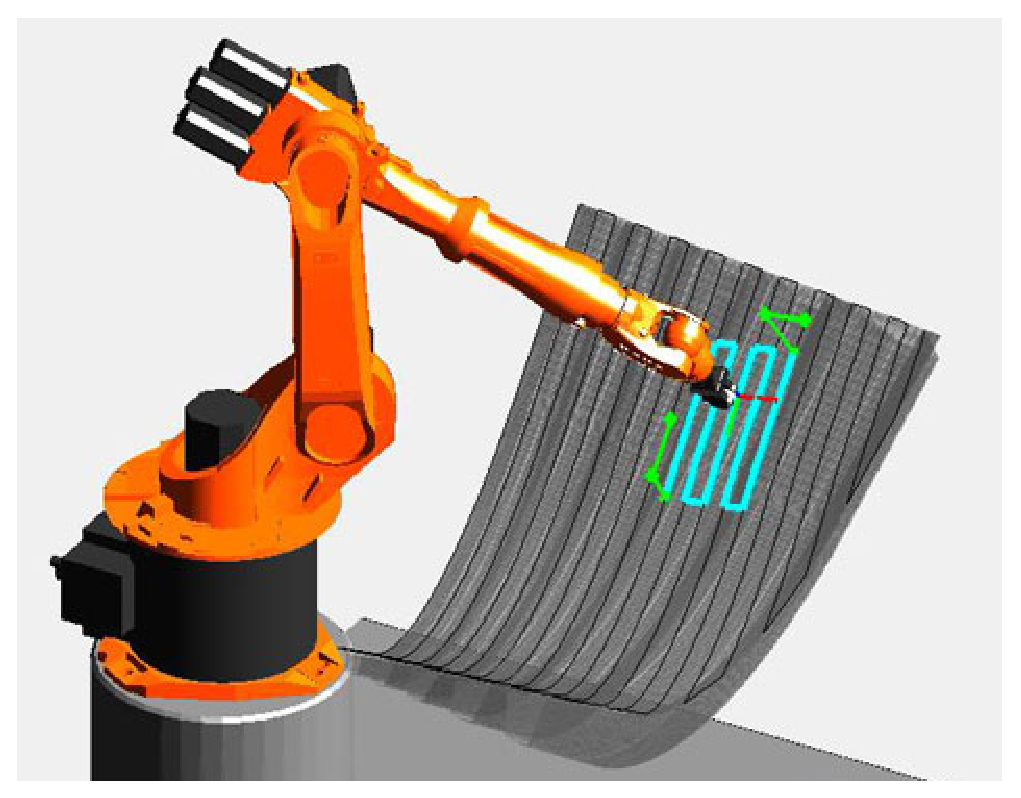
\includegraphics[scale=0.5]{img/chapter_1/example_coverage.eps}
	\vskip-15pt
	\caption*{\tiny twi-global.com}
	\caption{An example of an inspection coverage performed by a robotic arm.}
	\label{img:example_coverage}
\end{figure}

It is difficult to discuss good solutions to the coverage path planning problem because the notion of \emph{goodness} varies from one application to another. For example, a good coverage path for a painting robot would result in the most uniform paint layer on the surface. A good coverage path for a monitoring application would result in the entire area captured in high quality. Because of this, a body of existing solutions in literature are typically very specialized. On the other hand, there is a number of works in literature that focus on the theoretical analysis of the problem. These tend to propose solutions that theoretically achieve complete coverage; however, they fall short in practice.

In this work, we propose an approach that aims to make coverage paths more practical. The goal of the proposed solution is to compute a coverage path that is as \emph{straight} as possible. This is motivated by typical dynamics of robots. Vast majority of robotic systems are more efficient when a path between points $A$ and $B$ is a straight line segment. In other words, other paths that require turns are usually less efficient. Hence, a coverage path planner should minimize the number of turns in its paths. We approach this goal by studying paths with special structure called the segmented paths. These segmented paths consists of a sequence of pairs of straight and transitions line segments. With these paths, the goal of minimizing turns can be achieved by minimizing the number of straight line segments in the path with the condition that complete coverage is achieved. We then use these concepts to solve a more general $n$ robot coverage path planning problem. The goal of this problem is to compute $n$ coverage paths for a team of $n$ robots such that the entire workspace is covered.

\section{Thesis Contribution}
\label{section:thesis_contribution}

Our main contributions in this work are several. First, we design a metric called the altitude that aids with the computation of the number of lines required for full coverage. We introduce an algorithm for computing this metric for general polygons and propose a way to compute the minimum altitude for a given polygon. We then propose a greedy algorithm for decomposing the workspace into regions with the minimum overall altitude. The result of the algorithm is a workspace decomposition where the sum of minimum altitudes is minimized. One of the important aspects of the algorithm is a procedure for making minimum altitude cuts. This procedure is introduced and the proof of its correctness is provided. Lastly, we compute the coverage path by populating each cell with straight line segments and computing a tour of these lines. This tour is computed by framing the problem as a Generalized Travelling Salesman Problem. The computed tour is a complete coverage path. 

The focus of the second part of the thesis is an extension of the concepts developed for the single agent coverage to the multi-agent coverage. We propose a decoupled approach to this problem. The first subproblem deals with partitioning the workspace into $n$ cells such that the maximum cost amongst all cells is minimized. We propose a greedy algorithm for computing such a partition. This partition makes use of a metric that acts as an approximation to the true cost of a coverage path. The design and analysis of this metric is provided. The second subproblem involves solving the single agent coverage $n$ times for every robot in the team.

\section{Organization}
\label{section:organization}

The thesis is organized into six chapters. Chapter~\ref{chapter:literature_review} contains the literature review of single and multi-agent coverage works. Chapter~\ref{chapter:background} reviews some of the concepts used through out this thesis. Chapter~\ref{chapter:single_agent_coverage} introduces our approach to the single agent coverage path planning problem. Chapter~\ref{chapter:multi_agent_coverage} introduces our approach to the multi-agent coverage path planning problem. Finally, Chapter~\ref{chapter:future_work} provides conclusion to this thesis and recommendations for avenues of future research.

\end{document}